1.1
\begin{comment}
本研究では，日本の若者の自己開示の促進に焦点を当て，人間関係の親密化を支援するための方法論の確立を目的とする．この研究は，現代の若者が直面する人間関係の親密化の困難さに対して，実践的な解決策を提供することを目指すものである．
% todo:研究背景で目的を書くのは違う．〇〇を研究の対象とする．とかの方が適切かな

特に若年期は，新たな出会いの機会が豊富で，人間関係を構築・維持するのに最適な時期とされている．% todo:エビデンス
特に，自身の内面を他者に伝えるような深い自己開示は，関係性の親密化において重要な役割を果たす．自己開示は一般的に段階的に深まっていくプロセスをたどり，その過程で開示内容に対する他者からの受容が重要な役割を果たすことが知られている．

このように段階的に深まっていく自己開示は，同時に開示内容の広がりとも関係している．図1.3は，関係が親密化するにつれて開示内容の広がりと深さが共に増していく様子を示している．

\begin{figure}[H]
    \centering
    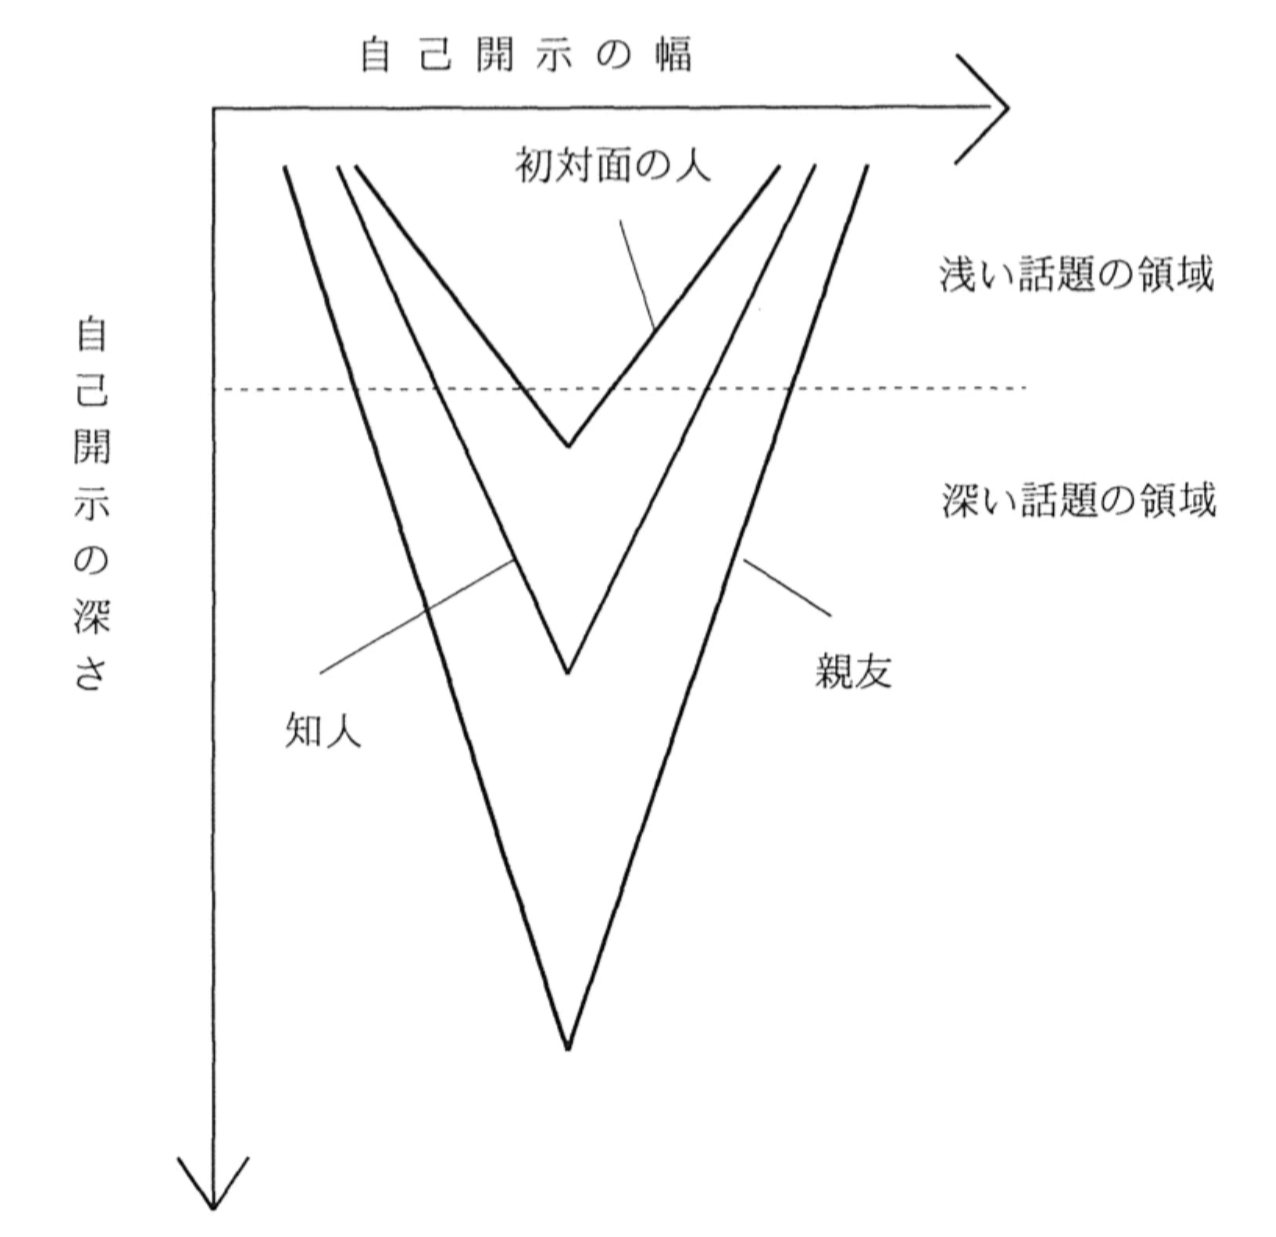
\includegraphics[width=0.5\linewidth]{image/自己開示_深さと広さ.png}
    \caption{社会的浸透過程における自己開示の深さと幅}
    \label{fig:自己開示_深さと広さ}
\end{figure}
\end{comment}

1.2
\begin{comment}
\subsection{親密度による自己開示のしやすさ}
ChaikinとDerlega\cite{chaikin_1974_A}\cite{chaikin_1974_B}の研究では，友人に対する自己開示が最も適切とみなされ，特に深い自己開示が好ましいとされる．一方，見知らぬ人に対する深い自己開示は不適切とみなされることが示されている．

\subsection{自己開示が親密化に及ぼす効果}\label{親密化}
% 類似性と親密性のはなし
研究では，自己開示には対人魅力を増加させる機能があることが報告されており，特に趣味などの類似性の確認が接触機会を増加させ，親密化を促進することが指摘されている．
自己開示を通じた相互の情報交換により，類似性・異質性の確認が促進され，そのプロセスを通じて親密化が進展するとされている．
% 引用：論文「親密化過程における自己開示機能の探索的検討 : 自己開示に対する願望・義務感の分析から」

% ＜親密度と自己開示の関係．適切性の観点＞
受容性（受容・拒絶）を考えるうえでは開示者と被開示者の親密性についても避けられない．自己開示の適切性は関係性の親密度によって異なるためである．榎本\cite{榎本_1997_自己開示の心理学的研究}はその一連の自己開示研究において，親友に対しては顔見知り程度の友人よりあらゆる側面で開示しやすく，話しやすい側面と話しにくい側面の開示料乖離が小さいと述べている．親密性は自己開示の量・内容および動機など全般に関わる大きな要因であり，受容性を考える際にも被開示者が開示者にとってどのような心理的距離を持つ相手であるかは重要な問題となりうる．


\subsection{自己開示の広さ}
% ただし，榎本\cite{榎本_1997_自己開示の心理学的研究}が述べるように，特定の話題領域の開示のみが深まっていったり，関係が深まるとともに開示内容の幅が狭まると言ったケースもあり得るため，この図の限界は心得ておく必要がある．研究において複数の話題を扱う場合，その話題に関する言及度合いは一律にする必要がある．例えば趣味に関する話題を1時間話し，私生活に関する話を30分話すのではそれぞれの話題での深さも異なるためである．よって，本研究においては1つの話題項目に着目し，話題領域である「広さ」の次元は扱わないものとする．


\subsection*{自己開示尺度}
% ＜自己開示尺度の話 → 趣味はレベル1 → ここに課題+アプローチ＞
丹羽・丸野\cite{自己開示尺度}は，日本の若者の自己開示の深さを測定する自己開示の尺度をAltman・Taylor（1973）の枠組みを参考に作成し尺度の精度を検討するために299人の大学生を対象に質問紙調査を行った．分析の結果，深さが異なる4つのレベルの自己開示を測定でき，開示する相手との関係性に応じて自己開示の深さが異なることを敏感に識別できた．また，親和動機および心理的適応度を測定する既存尺度から理論的に予想される結果においても，高い相関が見出され，妥当性の高い尺度であることが確認された．以下にその自己開示の尺度を示す．この尺度は自己開示の深さをレベルⅠから，レベルⅣまでの4段階で示している．

レベルⅠは，もっとも浅いレベルで，「趣味・趣向」を想定したものである．一般的な自分の好みについての情報で，特に社会的常識から逸脱する趣味ではない限り，人格を疑われたりすることはない．

レベルⅡは，「容易には克服できない困難な経験」を想定したものである．これは，自分がこれまで経験してきたつらい体験やそれをどう乗りこえてきたかに関する情報である．これらの情報は，開示者の性格特性そのものを直接的に言い表してはいないが，開示者の現在の性格特性に何らかの影響を及ぼしているものと考えられる．

レベルⅢは，自分自身の「決定的ではない欠点や弱点」を想定したものである．これは，それほど重要ではないが未熟と思われる自分自身の認知や情動の側面である．認知や情動は自分自身の人となりそのものを示す．そのため，このレベルの自己開示は自分がどんな人間であるかを直接的に相手に伝えている．ただし，この段階での望ましくない程度は，それを知ることによって開示者に対する評価が決定づけられるほど重要なものではなく，たとえ一時的に開示者に対する評価が下がった場合でも，開示者がそれについて後から言い訳をしたり，あるいは，それを補える自分の肯定的側面を強調したりすることで，開示者に対する否定的認識の修復が可能となる．

レベルⅣは，最も深いレベルで，自分の性格や能力の否定的側面を想定したものである．レベルⅢとは異なり，このレベルの自己開示は，それによって開示者は修復不可能なほど否定的に認識され，これまで構築してきた2者間の親密な関係性が脅かされる危険性をはらむ．このような危険性を考慮してもなお開示することは，開示者が被開示者に対して「非開示者はそれでもなお自分自身を受け止めてくれるだろう」という絶大な信頼感を持っていることを意味する．非開示者はこのようなメタメッセージを開示者から受け取り，2者間にはより親密な関係性が築かれると考えられる．

% ＜趣味の開示でも，個人的意味を含む場合は深い自己開示になりうる ということを書く＞
ここで，一見表層的に見える趣味の開示であっても，ある程度の関係性の友人であっても真に好きなこと・ものや，その詳細を開示できる人は少ないと考えられる．また，その内容に個人的な意味や価値観が含まれる場合は，深い自己開示として機能する可能性がある．例えば，音楽の好みは個人のアイデンティティを強く反映することがあり\cite{rentfrow_2006}，その開示には心理的なハードルがあると考えられる．これは，趣味の好みが個人によって大きく異なり，否定的な評価を受ける可能性があるためである．

% 話題の内容として，丹羽・丸野\cite{自己開示尺度}はレベルⅠに趣味・趣向を提示しているが，趣味の開示についてより検討が必要であると考える．本研究では，開示ハードルの低い趣味から入り深い自己開示を促進するきっかけづくりという方向性で行う．
% 本研究では自己開示項目として，趣味の共有に着目する．趣味は一般的に表層的な自己開示として捉えられるが，個人のアイデンティティや価値観を反映する重要な次元でもある．また，趣味は類似性・相違性を考慮しやすく，相互の受容性の向上が測りやすいという利点を持つ．


% ----- たぶんいらない↓ ------------

% ＜様々な理論を紹介する．社会的浸透理論，社会的交換理論，ジョハリの窓＞
自己開示に関する研究では，様々な理論的枠組みが提案されている．社会的交換理論（Social Exchange Theory）は，Homans（1958）によって提唱された社会心理学的パラダイムであり，人間関係を報酬とコストの観点から説明する画期的な分析枠組みである．Emerson（1976）が指摘するように，この理論の特徴は経済的な取引とは異なり，信頼関係や感情的なつながりといった定量化が困難な次元を含む点にあり，人々の相互作用を柔軟に捉えることを可能にした．また，この理論の中核的な概念である「成功の命題」や「価値の命題」は，人々の社会的行動がポジティブな結果や主観的価値に基づいて選択され，継続されることを実証的に示している．

ジョハリの窓（Johari Window）は，人間関係における自己認識と他者認識の相互作用を説明する心理学的モデルとして，Luft と Inghamによって1955年に考案された画期的な概念である．Chapman（2003）が指摘するように，このモデルは「開放の窓」「秘密の窓」「盲目の窓」「未知の窓」という4つの象限で構成され，自己開示と他者からのフィードバックを通じて個人の認識領域が変化していく過程を説明している\cite{chapman_2003_JohariWindow}．特に，Steinberg（2007）が論じたように，開放の窓を広げていく自己開示のプロセスは，人間関係における相互理解と信頼関係の深化に重要な役割を果たしている\cite{steinberg_2007}．

\begin{figure}[H]
    \centering
    \includegraphics[width=0.5\linewidth]{image/JohariWindow.png}
    \caption{ジョハリの窓 モデル}
    \label{fig:JohariWindow}
\end{figure}


\begin{comment} %類似性は使わないから，必要ないかも
\subsection{類似性と対人魅力}\label{}
% pin:この項では，類似性 → 相補性 が親密化において重要であることを示したい．そのプロセスというか，その段階を踏ませることが必要

自己開示の受容において，開示者と被開示者の類似性は重要な役割を果たす．「類は友を呼ぶ」という言葉どおり，自分に似た性質を持つ人に対して魅力を感じやすい．特に，価値観や趣味・興味の類似性は，相手への受容を促進する効果がある．


% ＜類似性ー対人魅力の視点から述べる＞
類似性に関する先行研究においては，Byrneをはじめとして類似性が対人魅力を増加させることが報告されている\cite{門田_2004_類似性}．奥田（1999）や相川\cite{相川充_2010}によれば，2者間で互いの態度が似ていると認知される場合，特に当人にとって重要な態度の類似性が認められる場合，相手に対する魅力が高まるという．また，松井（1993）は性格の類似性も一般に親密化に影響することを指摘している．


% ＜特に関係初期段階で，類似性が重要＞
類似性の影響は，特に関係構築の初期段階において顕著である．初対面の相手とのコミュニケーションでは，お互いの情報を手探りで引き出し，共通点を探すところから始まる．共通点が見つかると親近感が湧き，会話が大きく促進される．今川・岩淵（1981）によれば，相手を好ましいと思う場合，実際以上に類似性を感じる理想化傾向さえ生じるという．%  榎本のやつにあった


このように，人間関係の発展過程においては，初期段階での類似性の認知から，関係の親密化に伴う相補性の受容へと移行していくことが重要である．この段階的な変化を適切に支援することが，親密な関係の構築において不可欠となる．

% ＜相補性のメリットをいくつかの観点から述べる＞
しかし，関係が安定して深まるにつれて，互いに相手の態度や性格の異質性にも目が向くようになる．相川\cite{相川充_2010}は，「関係が親密になってからの異質性の認知は，自分と相手の違いを認め，違っているからこそ大切な相手だと受容し合う認知である」と述べている．

% ＜類似性の重要性の再確認＞
類似性の認知は，相手への親近感や安心感を生み出し，自己開示と受容の相互作用を促進する重要な基盤となる．特に関係初期において，共通点を見出すことは心理的な距離を縮め，その後の相補性の受容へとつながる重要な足がかりとなる．

% ＜近年の重要性＞
近年の日本社会では，相手の意見を頭ごなしに否定するのではなく，価値観の違う意見も取り入れるといった「相補性」の重要性が認識されている．例えば音楽の好みにおいて，自身と相手の趣味が合わない場合でも，「新しいジャンルかも！聴いてみようかな」「こういうのも好きなんだ．逆に私はこういうのをよく聴いているんだよね」と受容しつつ自己開示をしていく姿勢が求められる．

このように，持続的な関係性の構築においては，まず類似性に基づく信頼関係を築き，その上で相補性を受容していくという段階的なプロセスが重要となる．本研究では，この知見に基づき，類似性と相補性の両面を考慮した受容促進の方策を検討する．
\end{comment}



% ＜メリットとデメリットの対比＞
一方デメリットとして，，関係の初期段階における過度な自己開示は，関係性の発展を阻害する可能性がある．これは，過度の開示が心理的な不安定さの表れとして受け取られる可能性があるためである．その結果，自己開示が相手に受け入れられず，かえって関係性の悪化や拒絶につながるリスクがある．% エビデンス

% ＜性差について＞
さらに，自己開示には性差も存在する．榎本\cite{榎本_1997_自己開示の心理学的研究}は，非常に多くの研究から男性より女性の方が自己開示度が高いことを明らかにしている．一般的に男性より女性の方が深い自己開示をする傾向が見られ，相手から深い自己開示を引き出す．
また，開示の相手としては異性よりも同性の方が深い自己開示をしやすいことが知られている\cite{武田裕子_2013}．% 引用：論文「初級日本語クラスでの「個人化作文」における自己開示の深さの分析」p3


% ＜コミュニケーションの種類＞
コミュニケーションと言う用語は，日常生活で頻繁に使用される言葉である．しかし，コミュニケーションとは一義的に定義できる概念ではなく，多様な事象である．そこで，深田\cite{深田_2000}は，多数あるコミュニケーションの概念を以下の3つに大別した．

\begin{enumerate}
    \item 相互作用過程的概念タイプ：当事者が互いに働きかけ，応答し合う相互作用過程．コミュニケーションを通して相互理解と相互関係が成立すると考える立場
    \item 意味伝達過程的概念タイプ：一方から他方へと意味を伝達する過程．当事者はコミュニケーションを通して意味を共有できると考える立場
    \item 影響過程的概念タイプ；一方方法に対して影響を及ぼす過程．コミュニケーションを通して，人間は他社に影響を与える事ができると考える立場
\end{enumerate}

本研究においては，1.の「相互作用過程的概念タイプ」でかつ，個人間で行われるコミュニケーションである対人コミュニケーションを対象とする．これは，自己開示と受容の相互作用の状態を明示的に作り出し，観察・分析を行うためである．

% ＜いろいろ＞
深田\cite{深田_2000}によると，対人コミュニケーションの本質的特徴の1つは，2者間で交わされるコミュニケーションを基本とするのである．2つ目の特徴は，送り手と受け手が固定しておらず，当事者間で送り手の役割と受けての役割が交代すること．3つ目は，対面状況でのコミュニケーションが基本であるという点である．

% ＜システムが介入する場合でも，対人コミュニケーションの分野といえる理由にしたい＞
ただし，携帯電話といったパーソナル・メディアを介したコミュニケーションを対人コミュニケーションとみなす研究があるために，メディアが対人コミュニケーションにきたす次元も考慮にいれる必要がある．


% ＜関係の段階．友人関係や，中期段階．その定義＞ 
\end{comment}


1.3
\begin{comment}
% ＜深さや内容によって，受容性が変わる（自論）＞
開示内容の深さと広がりによって，受容の程度や質は異なる．表層的な自己開示は一般的に受容されやすい一方で，深い自己開示は被開示者に大きな心理的負担を与える可能性がある．また，開示内容が否定的内容である場合も受容に影響を与える要因である．社会的に受容されやすい内容は，被開示者からも受容されやすい傾向にある．

\end{comment}

\begin{comment}
\section{関連研究}

\ref{自己開示}節や，\ref{受容}節では，自己開示を段階的に行うことの重要性と，類似性から相補性に移行していくことが重要であると述べた．本節では，対人コミュニケーションにおいてそれらが実際にどのように支援されているかについて，既存研究から述べる．




\subsection{システムによるコミュニケーション支援}
% ＜色んなコミュニケーションに関する研究を示す＞
システムがどのようにコミュニケーションを改善するかについて様々な研究が行われている．コミュニケーション支援システムに関する研究は，支援対象とするコミュニケーションの種類や利用者の特徴によって大きく分類できる．例えば，ブレインストーミングなどの目的志向のコミュニケーションを支援する研究がある．具体的には，話題に関連する画像を提示することで具体的なアイデアを引き出すシステム\cite{wang_2010idea}や，壁面ディスプレイにアイデアをクリッピングすることでディスカッションを整理するシステム\cite{shi_2017_ideawall}などが提案されている．

次に，親睦を深めることを目的としたコミュニケーション支援システムがある．例えば，家族のコミュニケーションを活性化するために適切な写真を推薦するシステム\cite{brush_2008_family}や，食事の場を楽しくする情報を食卓に投影するシステム\cite{itou_2013_meat}が提案されている．また，初対面の話者を対象に，SNSから取得した互いの共通点を提示することで会話を促進し，親しさを向上させることを目的としたシステム\cite{nguyen_2015_sns}も提案されている．

% todo:もっと書き足してもいいね

% --------------------------------------------------------------------------------------------------------

\subsection{自己開示を促すコミュニケーション支援システム}

% 多分かきすぎ
自己開示を促すシステムについて，池田ら\cite{自己開示の促しによるコミュニケーション支援システム}は，初対面の話者間のコミュニケーションにおいて自己開示を促進することで親密度を高められるかという課題に取り組んだ．\ref{自己開示の概念}節で述べたように，社会心理学の知見では，話者同士の親密度が高まるとより深いレベルの自己開示が行われることが知られている．
しかし，システムによって自己開示を促進することで親密度が高まるかどうかについては，これまで十分な検証が行われていなかった．著者らは，この課題を検証するために以下の3つの仮説を設定した：

\begin{enumerate}
    \item コミュニケーションの話題として自己開示項目を提示することで親密度は向上する
    \item 自己開示の深さを考慮して開示に抵抗のある話題を避けつつ提示することで，システムの受容性を高めることができる
    \item 自己開示を促すシステムによる親密度の向上効果やシステムの受容性はユーザの性格に依存する
\end{enumerate}

これらの仮説を検証するため，池田らは自己開示項目を話題として提示するタブレット型のコミュニケーション支援システムを開発した．システムには，自己開示の深さを段階的に上げていく「段階手法」と，ランダムに話題を提示する「ランダム手法」の2つの方式を実装した．
192名の参加者による実験の結果，以下の知見が得られた：

\begin{enumerate}
    \item ランダム手法は支援なしの条件と比較して，有意に相手の印象を向上させることが確認された
    \item 段階手法はランダム手法と比較して，システムの受容性が高いことが示された
    \item ユーザの性格特性は，システムの効果に限定的な影響を与えることが確認された
\end{enumerate}

池田らは，自己開示をシステムが促進することで話者の親密度を高められることを 192 名の参加者による大規模な実験によって示した．また，心理学の知見を導入することで，自己開示のレベルを考慮して，開示に抵抗のある話題を避けつつ自己開示を促す段階手法を提案し，システムの受容性が高まることも示した．この研究は，コミュニケーション支援システムにおける自己開示の効果的な活用を探求した先駆的な取り組みといえる．

% ＜課題＞
しかしながら，システムへの過度な依存による自然なコミュニケーションの阻害や，固定的な話題提示タイミングによる会話の流れの分断，必要な場面に応じた適切な支援の欠如といった課題が存在する．

また，\ref{親密化}で述べたように，各自己開示項目には浅い開示から個人の性格や経験に関わる深い開示まで存在するが，これらの違いが十分に考慮されていない点も指摘できる．自己開示項目の深さの設定が単純化されており，同一項目内での開示レベルの違いへの考慮が不十分である．さらに，年代や文化による自己開示傾向の違いへの対応や，長期的な関係性構築における効果の検証も今後の課題として残されている．

既存のシステムを用いた親密化研究の多くは初対面での会話に焦点を当てており，既に親密な関係における研究は限定的である．また，段階的な自己開示を促す研究は池田ら以外にはほとんど存在せず，この分野には多くの未解明な部分が残されている．

これらより精緻化された段階的自己開示促進手法の開発や，自然な会話の流れに沿った支援方法の確立，より発展した関係性における効果的なアプローチの探求が今後求められる問題である．
\end{comment}